\section{Template-based geometry generation}

The geometry generation process begins with predefined Gmsh template files. These templates, which are created by the user, serve as the foundation for defining the problem-specific geometry. The template itself defines the problem being solved. 
A full example of a Gmsh template file used in this workflow can be found in Appendix \ref{appendix B}.

Each Gmsh template file incorporates placeholders for variable parameters, marked with the "DEFINE\_" string prefix (e.g., \texttt{DEFINE\_OFFSET}, \texttt{DEFINE\_ANGLE}). These placeholders are replaced programmatically with specific values provided by the optimization algorithm. Importantly, the number of placeholders in the template must correspond to the dimension of the optimization problem being solved, ensuring that each optimization parameter is appropriately mapped to a specific aspect of the geometry.

The Python function responsible for this substitution process is shown in Listing \ref{lst:template}. The function reads the template file, replaces the placeholders with the parameter values, and writes the modified geometry definition to a new file.

\newpage
\begin{lstlisting}[
language=Python,
caption={Function for modifying Gmsh template files.},
label={lst:template}]
def modify_geo_file(input_file_path, output_file_path, **kwargs):	
	# Open and read the content of the original GEO file
	with open(input_file_path, "r") as file:
		file_data = file.read()
	
	# Iterate through each keyword argument to replace placeholders
	for variable, value in kwargs.items():
		# Construct the placeholder string
		placeholder_variable = "DEFINE_" + variable.upper()
		replace_string = str(value)
	
	# Replace the placeholder with the actual value
	file_data = file_data.replace(placeholder_variable, replace_string)
	
	# Write the modified data to the new GEO file
	with open(output_file_path, "w") as file:
		file.write(file_data)
\end{lstlisting}

The modified Gmsh file is then processed to generate the desired geometry. Figure \ref{fig:outline} illustrates the geometry outlines produced by the template example from Appendix \ref{appendix B}. These outlines serve as the basis for further processing. Once the geometry outlines are defined, Gmsh is used to export the geometry as an \texttt{.stl} file. The \texttt{.stl} file captures the full 3D structure. Figure \ref{fig:stl file} shows the \texttt{.stl} file generated from the template example in Appendix \ref{appendix B}.

\begin{figure}[H]
	\begin{subfigure}{0.99\textwidth}
		\centering
		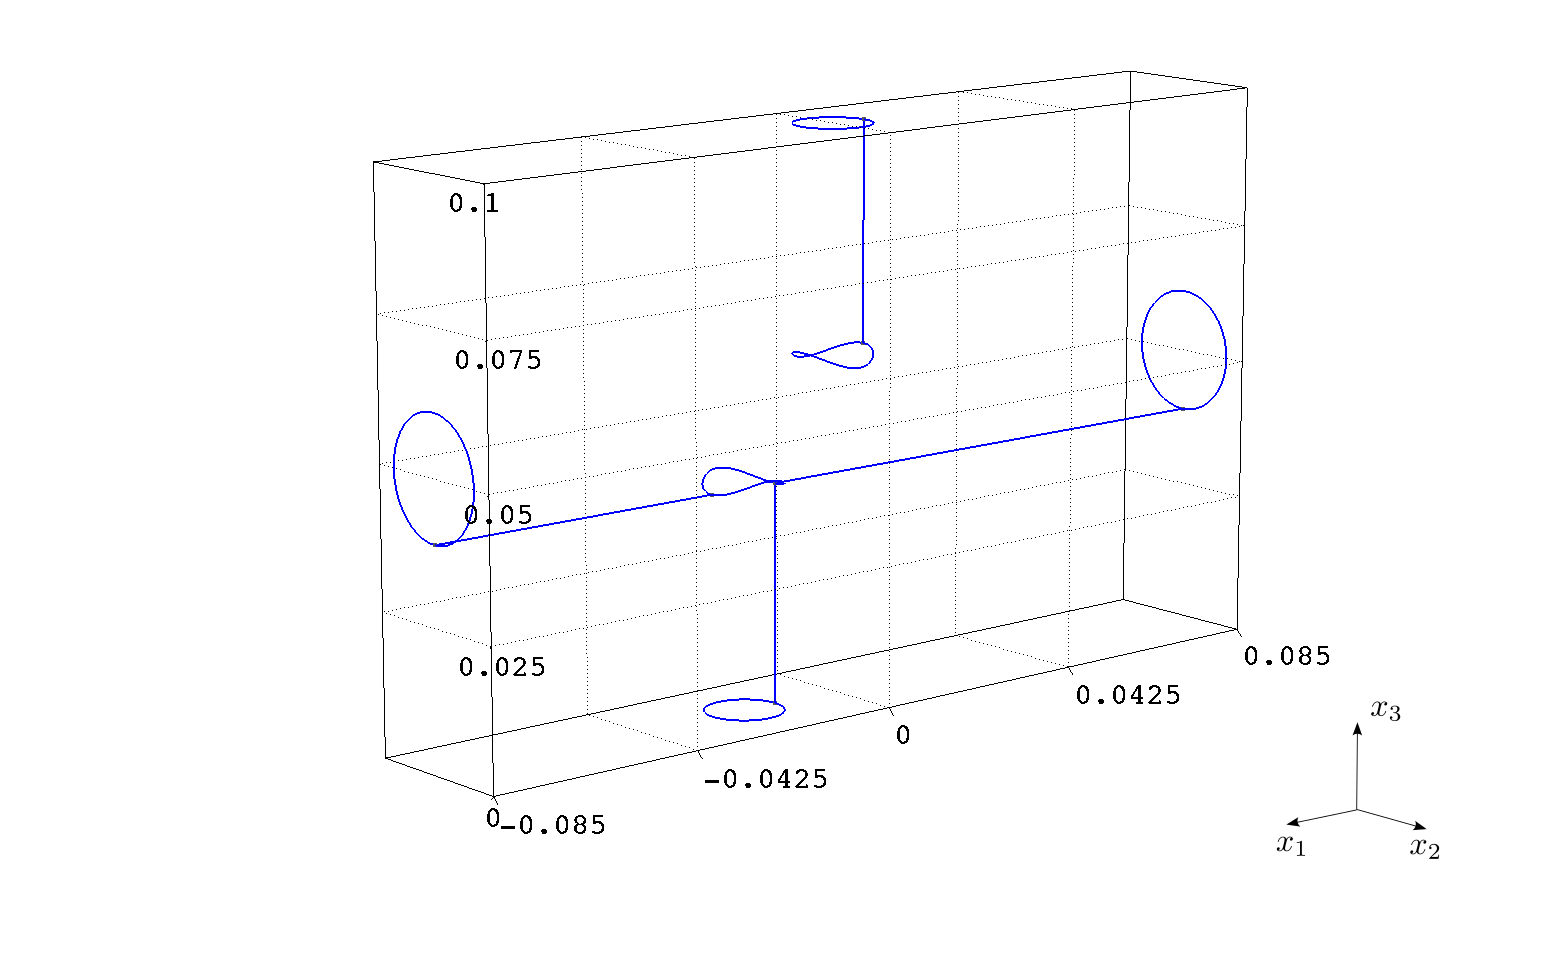
\includegraphics[width=0.83\textwidth, trim={70mm 25mm 10mm 10mm}, clip]{figures/outline.png}
		\caption{Geometry outlines generated using the Gmsh template.}
		\label{fig:outline}
	\end{subfigure}
\end{figure}
\begin{figure}[H]\ContinuedFloat
	\begin{subfigure}{0.99\textwidth}
		\vspace{-10mm}
		\centering
		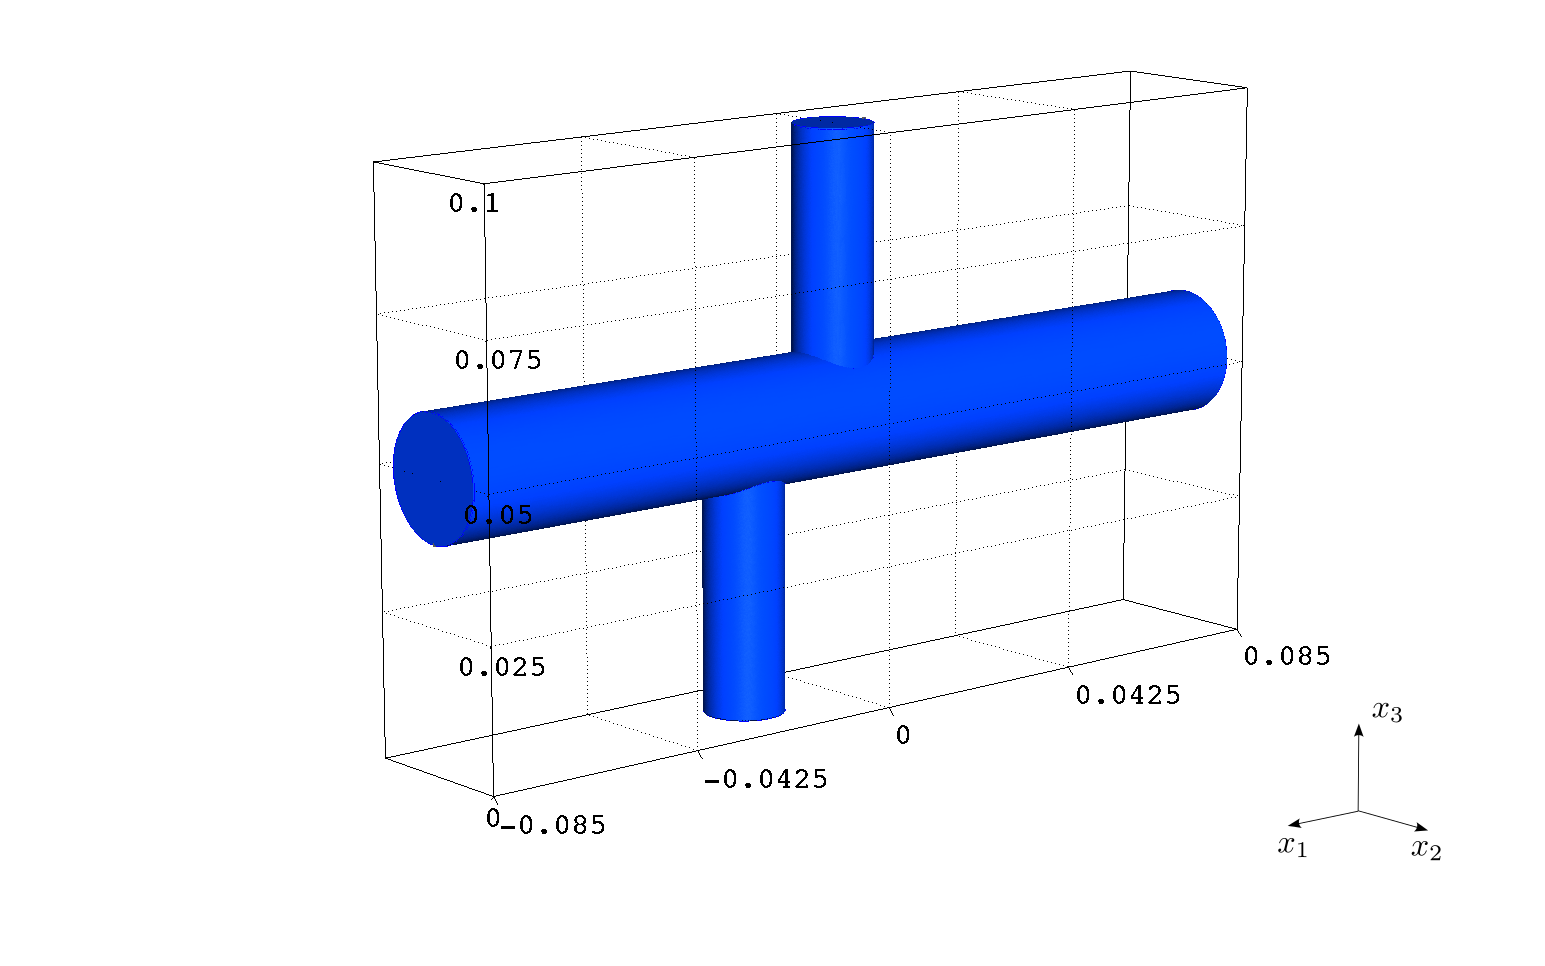
\includegraphics[width=0.83\textwidth, trim={70mm 25mm 10mm 10mm}, clip]{figures/stl.png}
		\caption{3D geometry exported to an \texttt{.stl} file. The blue volume represents the fluid sites later projected onto the LBM mesh.}
		\label{fig:stl file}
	\end{subfigure}
	\caption{3D geometry exported to an \texttt{.stl} file. The blue volume represents the fluid later projected onto the LBM lattice.}
\end{figure}
